\documentclass[runningheads]{llncs}
\usepackage{rotating,graphicx}
\usepackage{amsmath,amssymb}
\usepackage{booktabs,longtable,multirow}
\usepackage{float}
\usepackage{hyperref}
\usepackage{xcolor}
\usepackage{algorithm}
\usepackage{algorithmicx}

\setcounter{secnumdepth}{4}

\begin{document}

\title{Transformer-Based Fake News Detection: A Comparative Analysis of BERT, BiLSTM, and Hybrid Architectures Across Multiple Datasets}


\author{Md Akash Hossain\inst{1} and Parijata Majumdar \inst{2}}
\authorrunning{HOSSAIN, A. et al.}
\titlerunning{Transformer-Based Fake News Detection}
\institute{Department of Information Technology, Tripura University, Tripura, India\\
\email{hossainakash22958@gmail.com} \and
\email{parijatamajumdar@tripurauniv.ac.in}
}

\maketitle              % typeset the header of the contribution

\begin{abstract}
Fake news detection uses computing tools such as NLP and ML to identify and categorize fake or misleading information. Misinformation spreads through digital media and threatens public perception, democratic governance, and the reliability of information. This calls for automatic detection systems that can handle large volumes of data.

This paper proposes a layered model for fake news detection. It uses NLP for text preprocessing (noise reduction, tokenization, stopword elimination, and lemmatization), then feature extraction, and a comparison of several models.

Three models, a BiLSTM, BERT, and a hybrid BERT + BiLSTM, are evaluated on the ISOT and LIAR2 benchmark datasets with a single seed, three epochs, and headline-only input. On ISOT the three models reach 97.1\%, 97.7\%, and 98.2\% accuracy (F1 0.968, 0.974, and 0.980), and the hybrid is the best of them by a small margin. On LIAR2 they reach only 66.4\%, 68.9\%, and 68.2\% accuracy, with BERT slightly ahead. A further set of experiments on headline-only input evaluates a standalone GRU and four GRU-based hybrids (GRU+LSTM, GRU+CNN, GRU+BiLSTM, GRU+ResNet). All five reach 95.1--95.5\% accuracy and F1 scores between 0.9528 and 0.9560, and GRU+BiLSTM is the best of them.

A cross-dataset test on cleaned, deduplicated headlines qualifies these scores. Trained on ISOT, BERT reaches 0.984 accuracy on ISOT but only 0.504 on LIAR2, and the GRU behaves the same way. Transformer-based models are therefore the strongest within a dataset, but the models learn dataset-specific patterns, and detection across sources remains an open problem. The proposed system can be scaled for use in social media monitoring and fact-checking. Future work will add large language models and explainable AI.

\keywords{Fake news detection, Natural Language Processing, Machine Learning, Explainable AI, Misinformation.}
\end{abstract}

\section{Introduction}
\subsection{Background and Motivation}

Fake news detection is the automated task of identifying and categorizing false, misleading, or fabricated information that is presented as true news. It uses computational methods such as NLP and ML \cite{Shu2020FakeNewsNet,Shu2017FakeNewsDetection}. Digital media platforms have raised the amount of information generated and shared online to an unprecedented level.

This creates several problems: manipulation of public perception, interference with democratic processes, and loss of confidence in reliable sources \cite{Shu2020FakeNewsNet,Shu2017FakeNewsDetection}. Studies show that false information spreads faster on social media than real news \cite{Vosoughi2018Spread}. Reporters and fact-checkers cannot keep up with this pace and verify every item by hand.

The spread of disinformation can also have serious social and economic effects. Systems that detect fake news automatically are therefore an important research challenge.

\subsection{Types of Fake News}

``Fake news'' covers several classes of news items, each with different motives and features. The five main types are:

\begin{itemize}
\item \textbf{False News Stories:} Fabricated information designed to deceive readers.
\item \textbf{Manipulated News:} Real information that has been altered or distorted.
\item \textbf{Satirical News:} Absurd or exaggerated news that may be taken seriously.
\item \textbf{Clickbait:} News stories with misleading titles.
\item \textbf{Propaganda:} Biased or misleading information meant to shape perceptions or advance certain causes.
\end{itemize}

Because each class has its own characteristics, automatic detection is difficult. Detection needs models that can handle the meaning of the text and the contextual relationships within it.

\subsection{Role of Machine Learning and Deep Learning Methods}

Machine learning and deep learning work well for fake news detection because they can extract complex patterns from large datasets. Classical machine learning algorithms include Logistic Regression, Support Vector Machine (SVM), Naive Bayes, and Random Forest. Deep learning models such as LSTM and BiLSTM are built to identify sequences in text. Their effectiveness can still suffer when contextual associations are complex, especially with limited training data or too little training time.

Transformers such as BERT (Bidirectional Encoder Representations from Transformers) outperform earlier sequential models by producing bidirectional contextualized representations of text \cite{Kaliyar2021FakeBERT,Mehta2022RecentTrends}. Sequential models process text step by step, while BERT considers the whole input at once and so captures semantic relations more fully.

Text inputs are encoded numerically with methods such as TF-IDF, bag-of-words, Word2Vec, GloVe, and BERT embeddings. These encodings let models learn discriminative features for classification.

\subsection{Overview of the Proposed System}

The proposed fake news detection model is a multi-stage pipeline. It takes news input and ends with a detection result and a report. It accepts several input types: text, news headlines, and URLs of web pages that contain news articles.

The model is trained and tested on well-known benchmark datasets: LIAR, ISOT, and FakeNewsNet. They contain both real and fake news. Comparing results across datasets shows how well the models generalize.

An NLP preprocessing step cleans and normalizes the news text through tokenization, stop-word elimination, stemming, lemmatization, and lowercasing.

The feature extraction layer represents the text with TF-IDF, Bag-of-Words, Word2Vec, GloVe, and BERT's contextual embeddings. These representations capture both statistical and semantic properties of the text.

The classification layer was analyzed with several models: BiLSTM, BERT, and a combination of BERT + BiLSTM. On ISOT all three work well, and the BERT-based models are slightly ahead of the BiLSTM. On LIAR2 the scores are much lower and the differences are small. BERT + BiLSTM is the best model on ISOT, while BERT is the best on LIAR2.

Finally, the output layer labels the input as \textit{real} or \textit{fake} and gives a confidence estimate. A reporting mechanism produces an output that is easy to read.

\subsection{Contribution}

This study makes the following contributions:

\begin{itemize}
\item It proposes a multi-level architecture for fake news detection that combines NLP preprocessing, feature extraction, and classification.
\item It compares BiLSTM, BERT, and BERT + BiLSTM through experiments on several datasets.
\item It shows that transformer models are superior for fake news detection.
\item It benchmarks a standalone GRU against four GRU-based hybrid architectures (GRU+LSTM, GRU+CNN, GRU+BiLSTM, GRU+ResNet) under the same data split and training protocol.
\item It examines the drawbacks of sequential models and their hybrids under restricted training conditions.
\item It reports a cross-dataset evaluation showing that models scoring above 95\% on ISOT fall to about chance level on LIAR2.
\item It points to future research directions based on LLMs and XAI.
\end{itemize}


\subsection{Paper Organization}
The rest of the paper is organized as follows. Section 2 reviews related work on fake news detection with traditional machine learning, deep learning, and transformers. Section 3 explains the proposed system design. Section 4 covers the experiments, datasets, and results. Section 5 concludes the paper and describes future work.

\section{Related Work}

This section reviews nineteen peer-reviewed articles that form the basis of our research. They are grouped by theme, from traditional ML techniques to deep learning and transformers, and finally explainability and LLMs. Table \ref{tab:litreview} summarizes all of them.

\begin{longtable}{|p{0.19\textwidth}|p{0.19\textwidth}|p{0.18\textwidth}|p{0.18\textwidth}|p{0.18\textwidth}|}
\caption{Comparative Literature Review of Fake News Detection Methods} \label{tab:litreview} \\
\hline
\textbf{Contribution} & \textbf{Method} & \textbf{Advantage} & \textbf{Disadvantage} & \textbf{Future Scope} \\ \hline
\endfirsthead
\hline
\textbf{Contribution} & \textbf{Method} & \textbf{Advantage} & \textbf{Disadvantage} & \textbf{Future Scope} \\ \hline
\endhead
\hline
\multicolumn{5}{r}{\small\textit{Continued on next page\ldots}} \\
\endfoot
\hline
\endlastfoot
Introduced FakeBERT, a BERT-based deep learning model specifically designed for fake news detection on social media platforms with parallel CNN layers integrated into BERT architecture \cite{Kaliyar2021FakeBERT}. &
BERT + Parallel CNN layers for multi-scale feature extraction on LIAR and ISOT datasets \cite{Kaliyar2021FakeBERT}. &
Achieved 98.90\% accuracy; effectively captures contextual semantic relationships in text; outperforms traditional ML models significantly \cite{Kaliyar2021FakeBERT}. &
Computationally expensive; requires large GPU memory; limited to English language content only \cite{Kaliyar2021FakeBERT}. &
Extend to multilingual detection; reduce computational cost using model distillation techniques \cite{Kaliyar2021FakeBERT}. \\ \hline
Systematically compared multiple classical ML classifiers for fake news detection using linguistic and statistical text features extracted via TF-IDF \cite{Aphiwongsophon2021Detecting}. &
Logistic Regression, SVM, Naive Bayes, Random Forest with TF-IDF feature vectors on benchmark news datasets \cite{Aphiwongsophon2021Detecting}. &
Simple implementation; low computational cost; interpretable results; suitable for resource-constrained environments \cite{Aphiwongsophon2021Detecting}. &
Lower accuracy compared to deep learning; cannot capture semantic context or word order in text \cite{Aphiwongsophon2021Detecting}. &
Combine classical ML with deep learning features; incorporate metadata and social context signals \cite{Aphiwongsophon2021Detecting}. \\ \hline
Proposed a hybrid deep learning architecture combining CNN for local feature extraction and RNN for sequential pattern learning in news text \cite{Nasir2021FakeNews}. &
Hybrid CNN-RNN architecture with GloVe word embeddings trained on ISOT and FA-KES datasets \cite{Nasir2021FakeNews}. &
Captures both local and sequential text features simultaneously; better generalization than single-model approaches \cite{Nasir2021FakeNews}. &
Requires significant training data; slow inference time; struggles with short text like tweets and headlines \cite{Nasir2021FakeNews}. &
Apply to real-time social media streams; incorporate attention mechanisms for better interpretability \cite{Nasir2021FakeNews}. \\ \hline
Analyzed stylometric and linguistic style features that distinguish fake news from credible news using writing patterns and rhetorical structures \cite{Przybyla2020Capturing}. &
Stylometric analysis with SVM classifier; features include sentence length, punctuation patterns, readability scores on news datasets \cite{Przybyla2020Capturing}. &
Does not require external knowledge base; works purely on writing style; lightweight and fast inference \cite{Przybyla2020Capturing}. &
Style-based features are easily mimicked by sophisticated fake news creators; low robustness against adversarial content \cite{Przybyla2020Capturing}. &
Combine style features with semantic embeddings for more robust multi-feature detection systems \cite{Przybyla2020Capturing}. \\ \hline
Proposed evidence-aware fake news detection by retrieving external web evidence and combining it with claim credibility assessment using attention networks \cite{Popat2019DeClarE}. &
Attention-based LSTM with external web evidence retrieval and source credibility scoring on Snopes and PolitiFact datasets \cite{Popat2019DeClarE}. &
Incorporate external knowledge for verification; attention mechanism provides interpretability; better performance on political claims \cite{Popat2019DeClarE}. &
Dependent on external evidence availability; slow due to web retrieval; fails when evidence is unavailable or biased \cite{Popat2019DeClarE}. &
Integrate real-time knowledge graphs; improve evidence retrieval with more reliable fact-checking APIs \cite{Popat2019DeClarE}. \\ \hline
Developed a comprehensive fake news benchmark dataset incorporating news content, user social engagement, and spatiotemporal propagation features \cite{Shu2020FakeNewsNet}. &
Multi-modal dataset construction combining news text, social network graphs, user profiles, and publisher credibility on PolitiFact and GossipCop \cite{Shu2020FakeNewsNet}. &
Most comprehensive publicly available dataset; enables multi-modal detection research; includes social context signals \cite{Shu2020FakeNewsNet}. &
Dataset collection is time-consuming; social context features require platform API access which is increasingly restricted \cite{Shu2020FakeNewsNet}. &
Expand dataset to include video and image modalities; add multilingual fake news samples \cite{Shu2020FakeNewsNet}. \\ \hline
Surveyed state-of-the-art deep learning techniques for fake news detection covering transformer models, graph neural networks, and multi-modal approaches \cite{Mehta2022RecentTrends}. &
Systematic review of BERT, GPT, GNN, and multi-modal models across multiple benchmark datasets from 2017 to 2022 \cite{Mehta2022RecentTrends}. &
Comprehensive coverage of recent methods; identifies research gaps; provides clear taxonomy of detection approaches \cite{Mehta2022RecentTrends}. &
Survey only; no novel model proposed; coverage limited to English language studies \cite{Mehta2022RecentTrends}. &
Develop unified evaluation benchmark; explore cross-lingual and low-resource fake news detection \cite{Mehta2022RecentTrends}. \\ \hline
Combined BERT contextual embeddings with enhanced LSTM architecture for improved sequential and contextual understanding of fake news text \cite{Rai2022FakeNews}. &
BERT + enhanced LSTM hybrid model with attention mechanism trained on LIAR and ISOT datasets \cite{Rai2022FakeNews}. &
Superior performance over standalone BERT or LSTM; attention layer improves interpretability; robust to text length variations \cite{Rai2022FakeNews}. &
High model complexity; longer training time; requires substantial labeled data for effective fine-tuning \cite{Rai2022FakeNews}. &
Apply transfer learning to low-resource languages; integrate image features for multi-modal detection \cite{Rai2022FakeNews}. \\ \hline
Investigated psychological and cognitive bias patterns embedded in fake news content using computational linguistics and psycholinguistic feature analysis \cite{CarrascoFarre2022Fingerprints}. &
Psycholinguistic feature extraction using LIWC tool with ML classifiers; analysis of cognitive bias markers in fake vs.\ real news articles \cite{CarrascoFarre2022Fingerprints}. &
Novel perspective combining psychology and NLP; interpretable features; applicable across domains and languages \cite{CarrascoFarre2022Fingerprints}. &
Limited dataset size; psycholinguistic tools may not generalize across cultural and linguistic contexts \cite{CarrascoFarre2022Fingerprints}. &
Extend psycholinguistic analysis to social media posts; develop cross-cultural misinformation detection models \cite{CarrascoFarre2022Fingerprints}. \\ \hline
Proposed an optimized ensemble learning model using metaheuristic harmony search algorithm for automatic feature selection and classifier weight optimization \cite{Huang2020FakeNews}. &
Ensemble of SVM, RF, and LR optimized using Self-Adaptive Harmony Search metaheuristic algorithm on multiple news datasets \cite{Huang2020FakeNews}. &
Automatic feature selection reduces dimensionality; ensemble approach improves robustness; outperforms individual classifiers \cite{Huang2020FakeNews}. &
High computational overhead due to metaheuristic optimization; complex implementation; not suitable for real-time detection \cite{Huang2020FakeNews}. &
Apply neural architecture search for automated deep learning model optimization in fake news detection \cite{Huang2020FakeNews}. \\ \hline
Provided a foundational data mining perspective on fake news detection on social media, proposing taxonomy of detection methods including knowledge-based, style-based, propagation-based, and credibility-based approaches \cite{Shu2017FakeNewsDetection}. &
Survey and taxonomy of fake news detection approaches on social media platforms; analysis of linguistic, visual, and social context features \cite{Shu2017FakeNewsDetection}. &
Comprehensive taxonomy; covers diverse detection paradigms; foundational reference for the research community \cite{Shu2017FakeNewsDetection}. &
Survey only; no experimental results; limited coverage of deep learning and transformer-based models \cite{Shu2017FakeNewsDetection}. &
Develop end-to-end multi-modal systems combining all four detection paradigms for improved accuracy \cite{Shu2017FakeNewsDetection}. \\ \hline
Presented a comprehensive survey of fake news fundamental theories, detection methods, and future opportunities covering the full spectrum from fabrication to verification \cite{Zhou2020Survey}. &
Systematic review of knowledge-based, style-based, propagation-based, and credibility-based detection methods across multiple benchmark datasets \cite{Zhou2020Survey}. &
Thorough coverage of detection strategies; identifies open problems; provides structured framework for future research \cite{Zhou2020Survey}. &
Survey only; does not propose a novel detection model; limited coverage of multimodal and LLM-based approaches \cite{Zhou2020Survey}. &
Extend survey coverage to include graph neural networks, multimodal detection, and cross-lingual fake news models \cite{Zhou2020Survey}. \\ \hline
Proposed CSI (Capture, Score, Integrate), a hybrid deep learning model combining text content features with user behaviour and propagation patterns for fake news detection \cite{Ruchansky2017CSI}. &
Hybrid RNN model integrating article text (Capture), user response scoring, and propagation network modelling on CIKM benchmark dataset \cite{Ruchansky2017CSI}. &
First to integrate content, user, and propagation signals; significantly outperforms text-only baselines; applicable to social media platforms \cite{Ruchansky2017CSI}. &
Requires social engagement data which may be unavailable; complex multi-module architecture; limited generalization to non-social media news \cite{Ruchansky2017CSI}. &
Extend to real-time streaming data; integrate image and video modalities; explore graph-based propagation modelling \cite{Ruchansky2017CSI}. \\ \hline
Conducted a landmark empirical study on the spread of true and false news online across Twitter, revealing that false news spreads six times faster than true news and reaches more people \cite{Vosoughi2018Spread}. &
Large-scale analysis of 126,000 news stories tweeted by three million users over ten years; statistical modelling of diffusion cascades \cite{Vosoughi2018Spread}. &
Largest empirical study of its kind; provides strong motivation for automated fake news detection; highlights human-driven amplification of misinformation \cite{Vosoughi2018Spread}. &
Observational study; does not propose a detection model; limited to Twitter platform data \cite{Vosoughi2018Spread}. &
Extend analysis to other social media platforms; design detection systems that model propagation speed as a real-time detection signal \cite{Vosoughi2018Spread}. \\ \hline
Introduced the LIAR benchmark dataset containing 12,836 manually labelled short statements from PolitiFact with six fine-grained truthfulness labels for fake news detection research \cite{Wang2017Liar}. &
Benchmark dataset construction with metadata including speaker, subject, context, and party affiliation; baseline CNN and BiLSTM classifiers evaluated \cite{Wang2017Liar}. &
First large-scale manually labelled fake news dataset; enables fine-grained classification; metadata-rich annotations support multi-feature modelling \cite{Wang2017Liar}. &
Limited to political speech domain; fine-grained labels make classification harder; dataset may not generalize to social media news content \cite{Wang2017Liar}. &
Extend dataset with image and video evidence; develop cross-domain transfer learning models trained on LIAR for general fake news detection \cite{Wang2017Liar}. \\ \hline
Introduced LLaMA 2, a family of open-source large language models ranging from 7B to 70B parameters, enabling state-of-the-art language understanding and generation for downstream NLP tasks \cite{Touvron2023Llama2}. &
Open-source transformer-based LLM family fine-tuned for dialogue and instruction following; evaluated on multiple NLP benchmarks against GPT-4 and other proprietary models \cite{Touvron2023Llama2}. &
Freely available for research; competitive performance against closed models; enables privacy-preserving local deployment of large language models \cite{Touvron2023Llama2}. &
Requires significant GPU resources for inference and fine-tuning; may still produce hallucinations; limited multilingual capability compared to GPT-4 \cite{Touvron2023Llama2}. &
Fine-tune LLaMA 2 on fake news datasets; integrate with RAG pipelines to enable evidence-grounded fake news classification \cite{Touvron2023Llama2}. \\ \hline
Proposed Retrieval-Augmented Generation (RAG), a framework combining parametric knowledge of pre-trained LLMs with non-parametric retrieval from external knowledge bases for knowledge-intensive NLP tasks \cite{Lewis2020RAG}. &
RAG model combining dense passage retrieval with a sequence-to-sequence generator; evaluated on open-domain QA, fact verification, and knowledge-grounded dialogue tasks \cite{Lewis2020RAG}. &
Enables LLMs to access up-to-date external evidence; reduces hallucination; improves factual accuracy without full model retraining \cite{Lewis2020RAG}. &
Retrieval quality is highly dependent on the quality and coverage of the knowledge base; increased inference latency due to retrieval step \cite{Lewis2020RAG}. &
Apply RAG to fake news detection by grounding classification decisions in retrieved evidence from verified fact-checking databases \cite{Lewis2020RAG}. \\ \hline
Proposed LIME (Local Interpretable Model-agnostic Explanations), a technique for explaining the predictions of any black-box classifier by approximating it locally with an interpretable model \cite{Ribeiro2016LIME}. &
Model-agnostic local surrogate modelling using perturbed samples to identify which input features most influenced a specific prediction across text, image, and tabular data \cite{Ribeiro2016LIME}. &
Works with any classifier regardless of architecture; provides human-readable explanations; enables trust and debugging of black-box ML models \cite{Ribeiro2016LIME}. &
Local explanations may not reflect global model behaviour; computationally expensive for large input spaces; sensitive to perturbation sampling strategy \cite{Ribeiro2016LIME}. &
Apply LIME to explain fake news classification decisions; integrate with BERT-based models to highlight which words drove the REAL or FAKE prediction \cite{Ribeiro2016LIME}. \\ \hline
Proposed SHAP (SHapley Additive exPlanations), a unified framework for interpreting model predictions using Shapley values from cooperative game theory to quantify each feature's contribution \cite{Lundberg2017SHAP}. &
Unified additive feature attribution method grounded in Shapley values; applied to tree-based models, deep learning, and linear models for consistent global and local explanations \cite{Lundberg2017SHAP}. &
Theoretically grounded in game theory; consistent and locally accurate; enables both global feature importance and individual prediction explanations \cite{Lundberg2017SHAP}. &
Computationally expensive for large feature spaces and deep models; requires careful interpretation; may not capture feature interaction effects completely \cite{Lundberg2017SHAP}. &
Apply SHAP to quantify word-level contributions in BERT fake news classifiers; combine with attention maps for multi-level explainability dashboards \cite{Lundberg2017SHAP}. \\ \hline
\end{longtable}

\subsection{Motivation for using the Combined BERT + BiLSTM Model}

The reason for using BERT and BiLSTM together is not that BiLSTM performs poorly alone. The two models have complementary strengths. BERT is excellent at analyzing context and semantics. Its bidirectional transformer design captures such relationships, but it does so through attention and not through sequence modelling as RNNs do.

The BiLSTM is built to model sequences and captures temporal dependencies in text. It processes its input from left to right and from right to left.

In the proposed hybrid framework, BERT acts as a contextual feature extractor that produces informative token embeddings. The entire sequence of contextual embeddings from BERT, and not only the [CLS] token, is fed into the BiLSTM layer. The network can thus refine these contextual embeddings by adding the dependency aspect through the BiLSTM.

The resulting BERT + BiLSTM framework is designed to benefit from both contextual embeddings (BERT) and sequential learning (BiLSTM).

\section{Proposed System Architecture}

\begin{figure}[H]
    \centering
    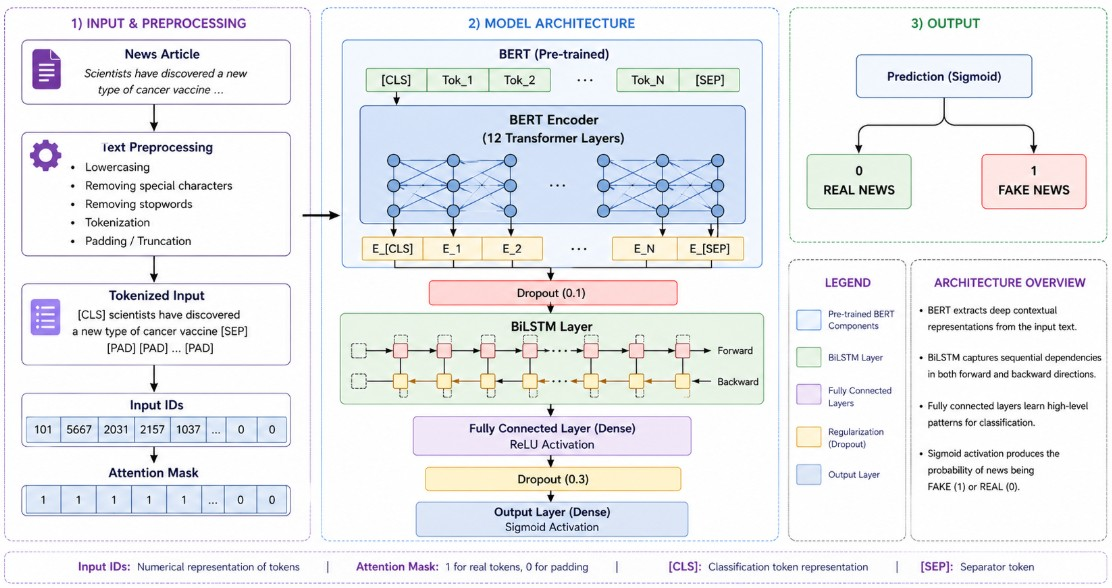
\includegraphics[width=\textwidth]{figures/Arch.jpg}
    \caption{Fake News Detection using BERT+BiLSTM model}
    \label{fig:architecture}
\end{figure}

The proposed detection system is a pipeline that converts unstructured news input into a classified output. The first stage is a user input layer that accepts text, a headline, or a link. A data collection layer then gathers the required data from benchmark datasets and, where possible, web sources. The collected data are stored in repositories for later training and testing.

Next, the NLP pre-processing module converts the unstructured text into a normalized form by tokenizing, removing stopwords, and lemmatizing. The feature extraction layer converts the text into numeric data with techniques such as TF-IDF and contextual embeddings such as BERT. In the classification layer, several classification algorithms are tested and evaluated, and BERT performs best.

Algorithm 1 shows fake news detection with the BERT + BiLSTM model.

\begin{algorithm}[H]
\caption{Fake News Detection using BERT + BiLSTM}
\begin{algorithmic}[1]
\State Input: Raw news text $T$
\State Preprocess text (tokenization, stopword removal, normalization)
\State Convert text into BERT embeddings
\State Extract sequence of hidden states from BERT
\State Pass embeddings to BiLSTM layer
\State Apply fully connected layer with Softmax
\State Output classification: REAL or FAKE
\end{algorithmic}
\end{algorithm}

\section{Experimental Results and Discussion}

The proposed framework is evaluated with four standard metrics from NLP and IR studies. They are defined as follows:

Accuracy is the share of all instances that are classified correctly:
\[
\text{Accuracy} = \frac{TP + TN}{TP + TN + FP + FN}
\]

Precision is the share of instances identified as fake news that really are fake:

\[
\text{Precision} = \frac{TP}{TP + FP}
\]

Recall is the share of actual fake news articles that the algorithm identifies:
\[
\text{Recall} = \frac{TP}{TP + FN}
\]

The F1-Score is the harmonic mean of precision and recall. It gives a balanced view and is particularly helpful under class imbalance:
\[
\text{F1-Score} = 2 \times \frac{\text{Precision} \times \text{Recall}}{\text{Precision} + \text{Recall}}
\]

Here TP = True Positive, TN = True Negative, FP = False Positive, and FN = False Negative. The confusion matrix is also used to evaluate the classification results.

Table \ref{tab:hyperparameters} lists the hyperparameters of each model. Each model was trained with hyperparameters suited to its architecture so that the comparison is fair. The BERT-based models are already pre-trained, so they use lower learning rates and small batches, while the BiLSTM uses a high learning rate. The combined model joins BERT embeddings with a BiLSTM layer.

\begin{table}[H]
\centering
\caption{Hyperparameter Configuration of Models}
\label{tab:hyperparameters}
\small
\begin{tabular}{|l|c|c|c|}
\hline
\textbf{Hyperparameter} & \textbf{BiLSTM} & \textbf{BERT} & \textbf{BERT + BiLSTM} \\ \hline
Embedding Type & GloVe & BERT Base & BERT Base \\ \hline
Max Sequence Length & 200 & 256 & 256 \\ \hline
Hidden Units & 128 & --- & 128 \\ \hline
Number of Layers & 2 & 12 (Transformer) & 12 + BiLSTM \\ \hline
Dropout Rate & 0.5 & 0.1 & 0.3 \\ \hline
Batch Size & 32 & 16 & 16 \\ \hline
Learning Rate & 0.001 & 2e-5 & 2e-5 \\ \hline
Optimizer & Adam & AdamW & AdamW \\ \hline
Epochs & 3 & 3 & 3 \\ \hline
Loss Function & Binary Crossentropy & Crossentropy & Crossentropy \\ \hline
\end{tabular}
\end{table}

The experiments use three benchmark datasets (Table \ref{tab:datasets}): LIAR \cite{Wang2017Liar}, ISOT \cite{ISOTDataset}, and FakeNewsNet \cite{Shu2020FakeNewsNet}. A Kaggle-hosted version of these datasets was used.

\begin{table}[h]
\centering
\caption{Dataset Description}
\label{tab:datasets}
\begin{tabular}{|l|c|c|c|l|}
\hline
\textbf{Dataset} & \textbf{Total Samples} & \textbf{Real News} & \textbf{Fake News} & \textbf{Source} \\ \hline
LIAR & 12,836 & 6,418 & 6,418 & PolitiFact Statements \\
ISOT & 44,919 & 21,417 & 23,502 & Reuters \& Fake News Sites \\
FakeNewsNet & 23,196 & 11,941 & 11,255 & PolitiFact \& GossipCop \\ \hline
\end{tabular}
\end{table}

The figures and tables in this subsection come from one set of runs on ISOT and LIAR2 (seed 0, a stratified 70:15:15 split, headline-only input, maximum length 64, batch size 32). The BiLSTM used randomly initialized embeddings over BERT WordPiece ids and not pre-trained GloVe vectors, so it differs from the hyperparameter table in embedding source and sequence length. The weights with the lowest validation loss were restored before testing. Earlier drafts of this paper reported a BiLSTM at 50\% accuracy and BERT and BERT + BiLSTM at identical 95\% scores. Those numbers did not reproduce in this rerun and have been replaced.


Table \ref{tab:comparison} gives the test results of the three models on ISOT. For a fair comparison, all three were trained for 3 epochs under the same conditions. The loss column is the test loss.

\begin{table}[h]
\centering
\caption{Performance Comparison of Fake News Detection Models}
\label{tab:comparison}
\small
\begin{tabular}{p{0.18\textwidth}ccccccp{0.18\textwidth}}
\hline
 \textbf{Model} & \textbf{Final Loss} & \textbf{Accuracy} & \textbf{Precision} & \textbf{Recall} & \textbf{F1 Score} \\ \hline
 BiLSTM & 0.0788 & 0.9714 & 0.9846 & 0.9523 & 0.9682 \\ 
 BERT & 0.0770 & 0.9768 & 0.9886 & 0.9603 & 0.9742 \\ 
 BERT + BiLSTM Model & 0.0657 & 0.9815 & 0.9914 & 0.9679 & 0.9795 \\ \hline
\end{tabular}
\end{table}

Table \ref{tab:comparison_extended} compares the models on the two benchmark datasets (ISOT and LIAR2). The models separate ISOT well and reach much lower scores on LIAR2.

\begin{table}[h]
\centering
\caption{Performance Comparison Across Multiple Datasets}
\label{tab:comparison_extended}
\small
\begin{tabular}{cccccc}
\hline
\textbf{Dataset} & \textbf{Model} & \textbf{Accuracy} & \textbf{Precision} & \textbf{Recall} & \textbf{F1 Score} \\ \hline
LIAR2 & BiLSTM & 0.664 & 0.685 & 0.771 & 0.726 \\
LIAR2 & BERT & 0.689 & 0.763 & 0.669 & 0.713 \\
LIAR2 & BERT+BiLSTM & 0.682 & 0.754 & 0.665 & 0.707 \\ 
ISOT & BiLSTM & 0.971 & 0.985 & 0.952 & 0.968 \\
ISOT & BERT & 0.977 & 0.989 & 0.960 & 0.974 \\
ISOT & BERT+BiLSTM & 0.982 & 0.991 & 0.968 & 0.980 \\ \hline
\end{tabular}
\end{table}

The standalone BiLSTM did well on ISOT, with 0.9714 accuracy, 0.9846 precision, 0.9523 recall, and an F1-score of 0.9682. It converged without trouble (test loss 0.0788), so the weak BiLSTM result of the earlier draft is not supported. On LIAR2 it reached only 0.664 accuracy, with high recall (0.771) and modest precision (0.685), which means it leans toward predicting the fake class.

BERT improved on the BiLSTM on both datasets, with 0.9768 accuracy and an F1-score of 0.9742 on ISOT (test loss 0.0770) and 0.689 accuracy and an F1-score of 0.713 on LIAR2. The gain over the BiLSTM is about 0.5 points on ISOT and 2.5 points on LIAR2, which is small. Language pre-training seems to help most where the text is hard, but a single seed cannot show that the differences are reliable.

The combination of BERT and BiLSTM was the best model on ISOT, with 0.9815 accuracy, 0.9914 precision, 0.9679 recall, an F1-score of 0.9795, and the lowest test loss (0.0657). On LIAR2 it scored 0.682 accuracy and an F1-score of 0.707, slightly below BERT alone. The BiLSTM head therefore gave a small gain on the easy dataset and none on the hard one.

Table \ref{tab:comparison_extended} shows that the ranking is not the same on the two datasets. This is a within-dataset result, and it comes from one seed, so differences of less than about one point should not be over-read. The cross-dataset test later in this section shows that the high ISOT scores do not carry over from one dataset to another.

The hybrid beat BERT alone on ISOT by about 0.5 points of accuracy and did not beat it on LIAR2. The BiLSTM module sits on top of BERT's contextual embeddings to detect sequences in the data. Its value may depend on the dataset, and multiple seeds and tuned hyperparameters are needed to confirm any gain.

The plots below were generated from the real test-set predictions and training histories of the runs reported in Tables \ref{tab:comparison} and \ref{tab:comparison_extended}. The scripts that produce them are \texttt{train\_three\_models.py} and \texttt{make\_figures.py} in the repository.

The confusion matrix compares predicted class values with actual values and has four elements: TP, TN, FP, and FN. It shows how the model behaves beyond accuracy alone. In fake news detection, the goal is to reduce false positives, where real news is classified as fake, and also to avoid false negatives, where fake news goes undetected. Fig. 2 shows the confusion matrices of BERT, BiLSTM, and BERT+BiLSTM for all datasets.

\begin{figure}[htbp]
\centering
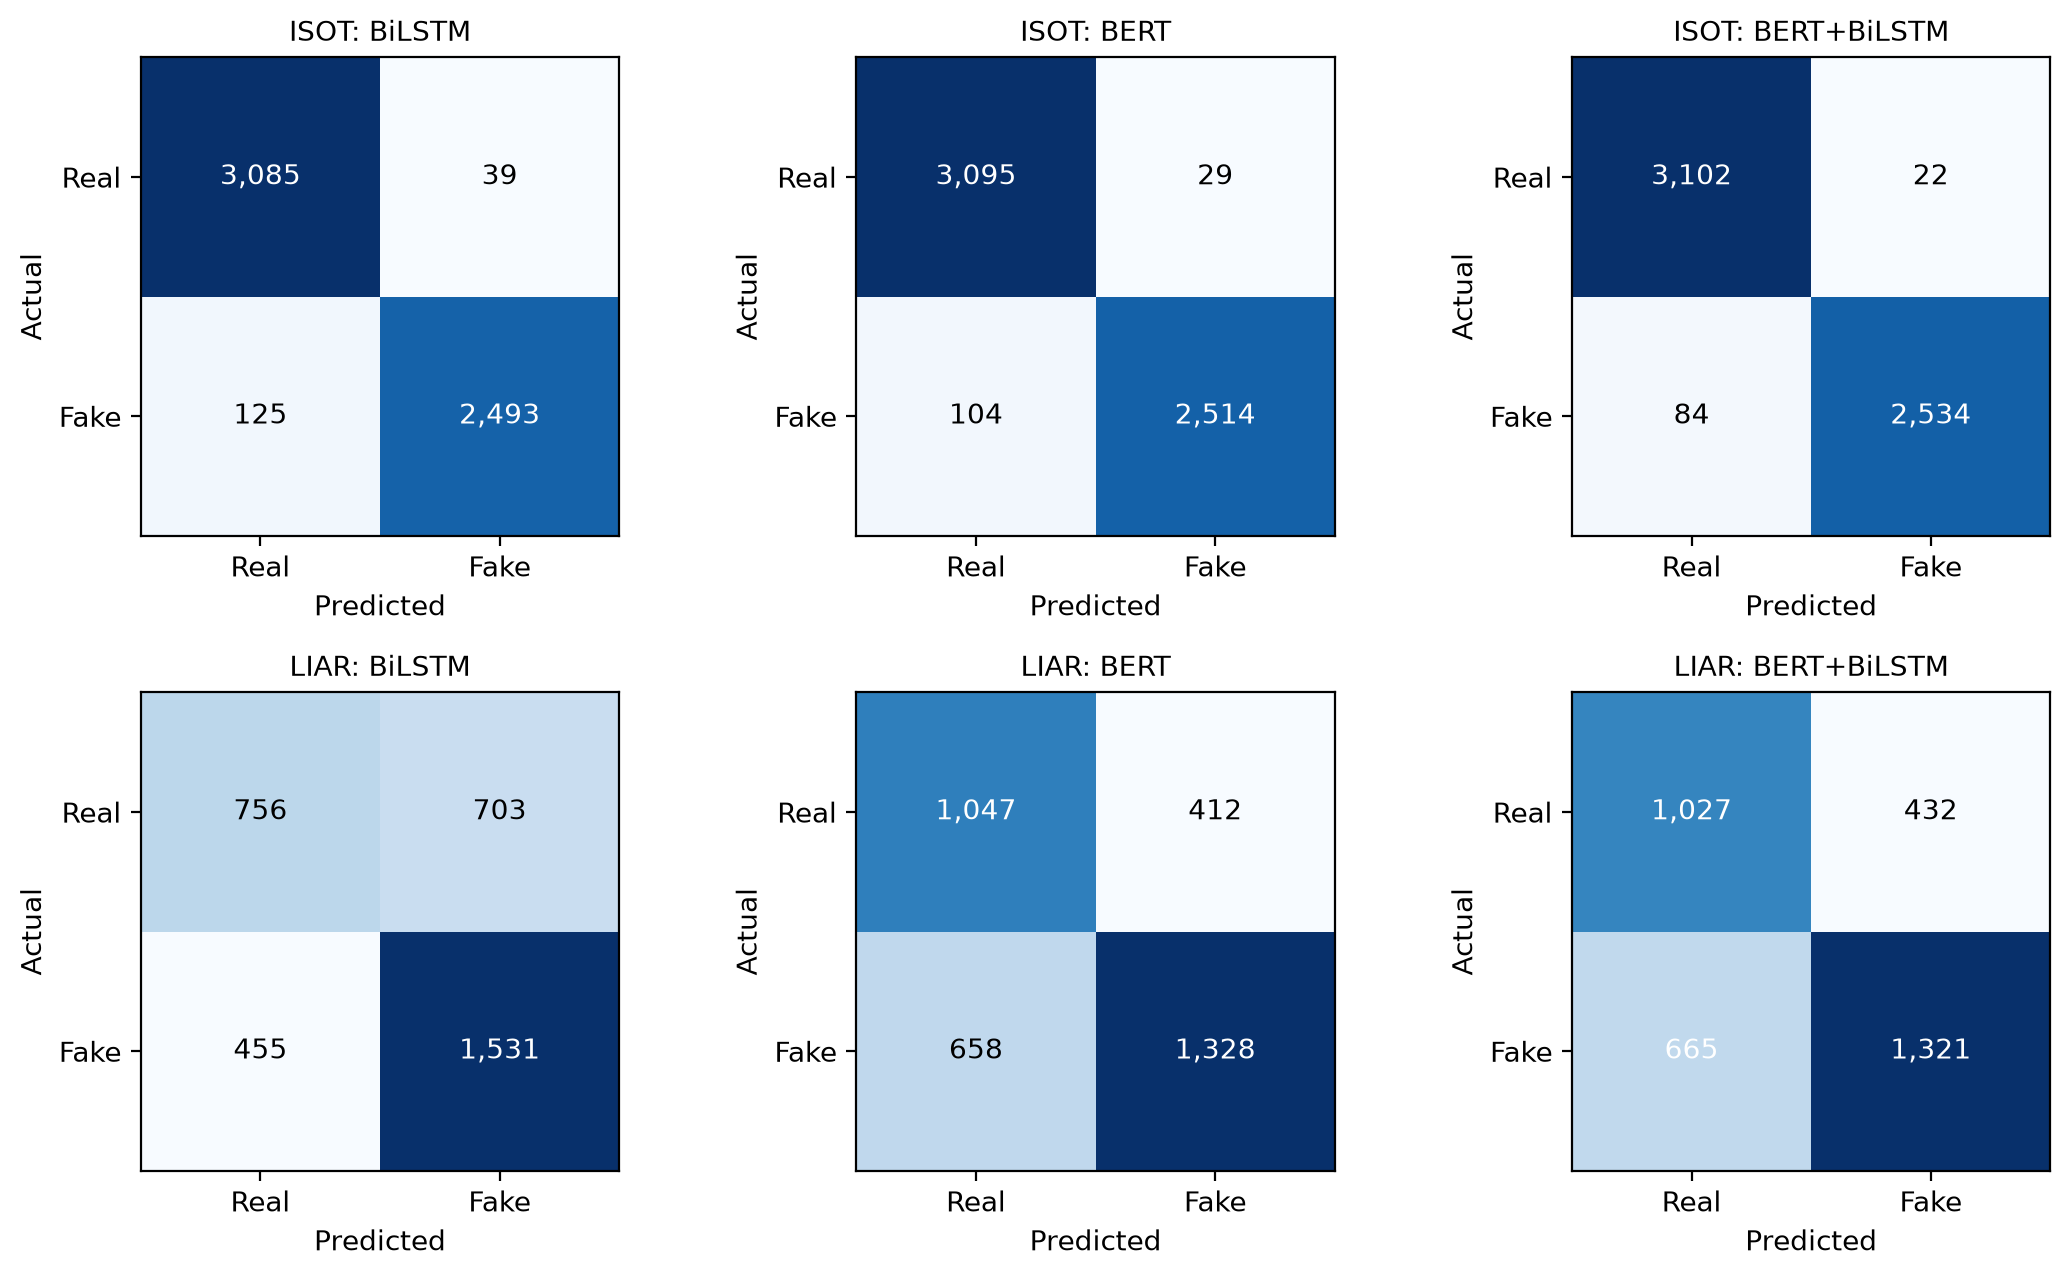
\includegraphics[width=0.88\textwidth]{figures/Confusion.png}
\caption{Confusion Matrix for BERT, BiLSTM and BERT+BiLSTM Model for all the datasets}
\label{fig:confusion}
\end{figure}

The ROC curve plots the True Positive Rate (sensitivity) against the False Positive Rate over various classification thresholds and shows how well the model separates true from false news. The closer the curve lies to the top left, the better the model. The area under the curve (AUC) summarizes discrimination in one number: values near 1.0 mean a very good classifier and 0.5 means a random one. The BERT-based models have the higher AUC on both datasets (ISOT 0.998 and 0.999 against 0.996 for the BiLSTM, LIAR2 0.769 and 0.763 against 0.721), although on ISOT the gap is small. Fig. 3 shows the ROC curves of BERT, BiLSTM, and BERT+BiLSTM for all datasets.

\begin{figure}[htbp]
\centering
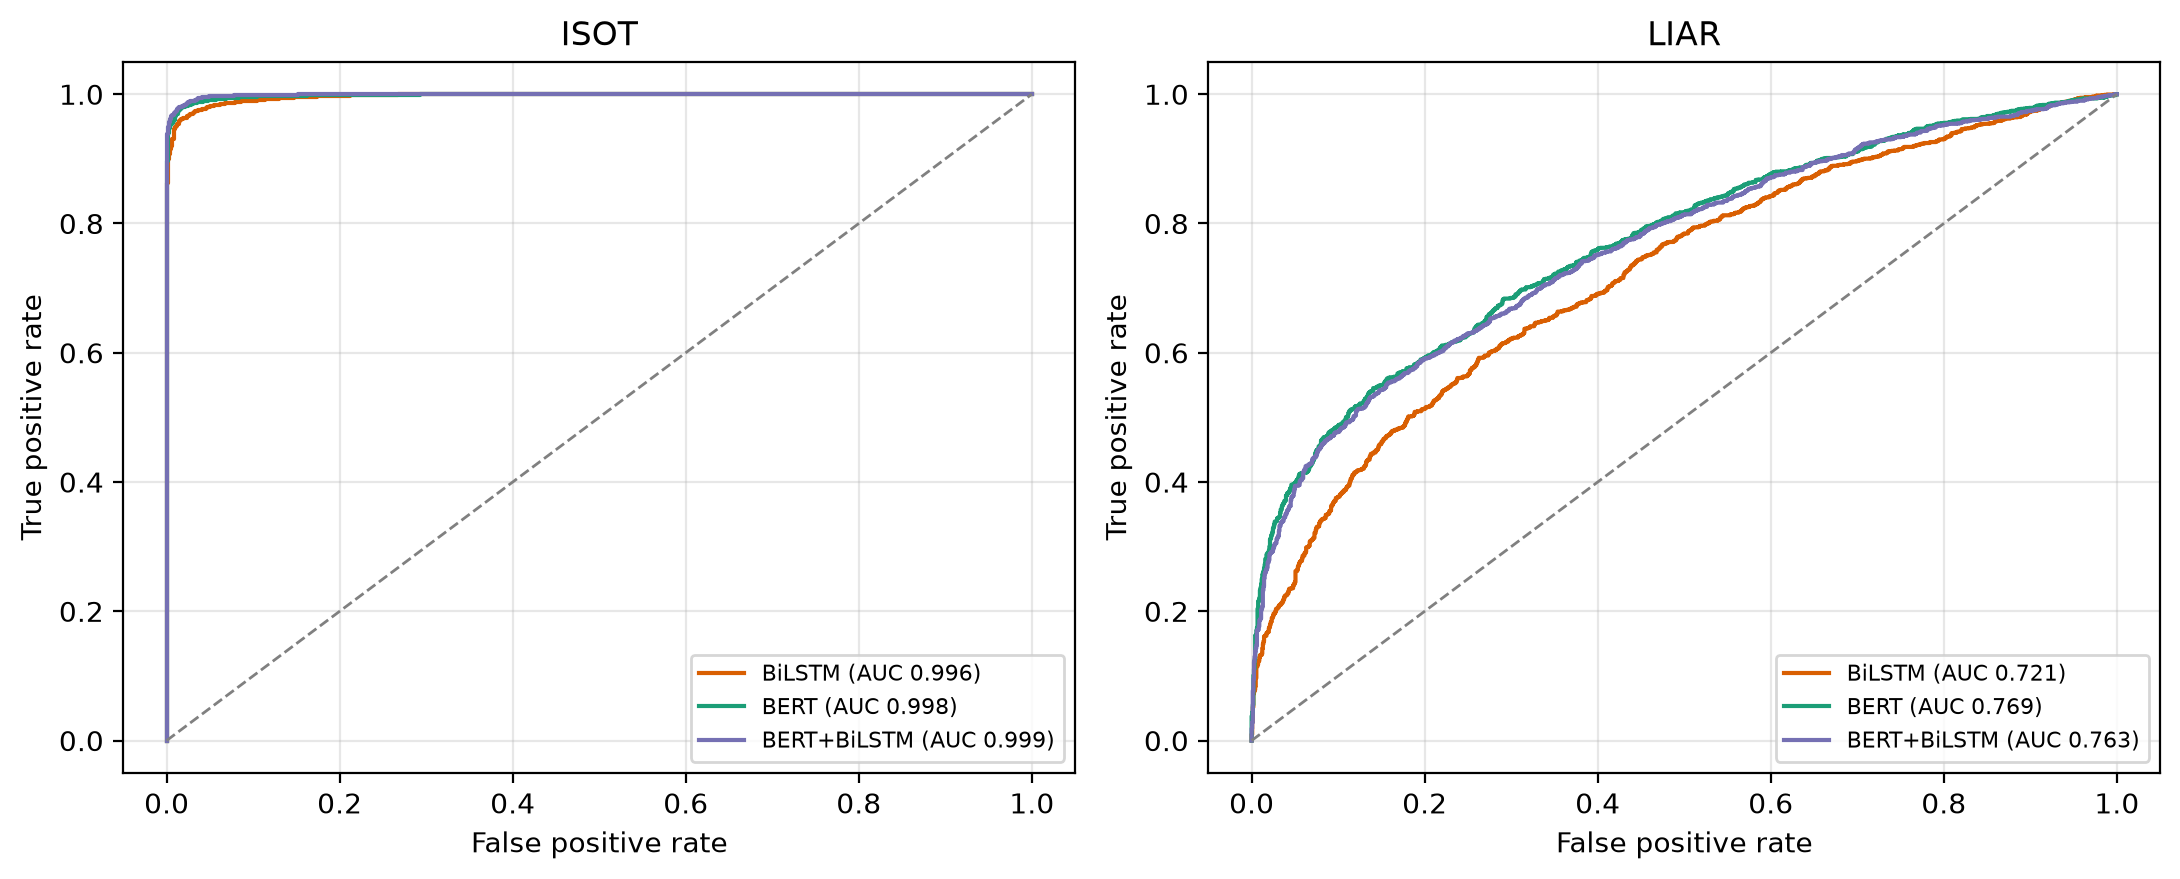
\includegraphics[width=\textwidth]{figures/ROC.png}
\caption{ROC Curves for BERT, BiLSTM and BERT+BiLSTM Model for all the datasets}
\label{fig:roc}
\end{figure}

The Precision--Recall (PR) curve shows the trade-off between precision and recall over different thresholds and is particularly relevant for skewed data. Precision is the share of predicted fake news that is truly fake, and recall is the share of actual fake news that the algorithm detects. An ideal model has both high, which the PR curve helps to identify. In fake news detection, high recall keeps false negatives low, and high precision keeps false positives low. Fig. 4 shows the PR curves of BERT, BiLSTM, and BERT+BiLSTM for all datasets.

\begin{figure}[htbp]
\centering
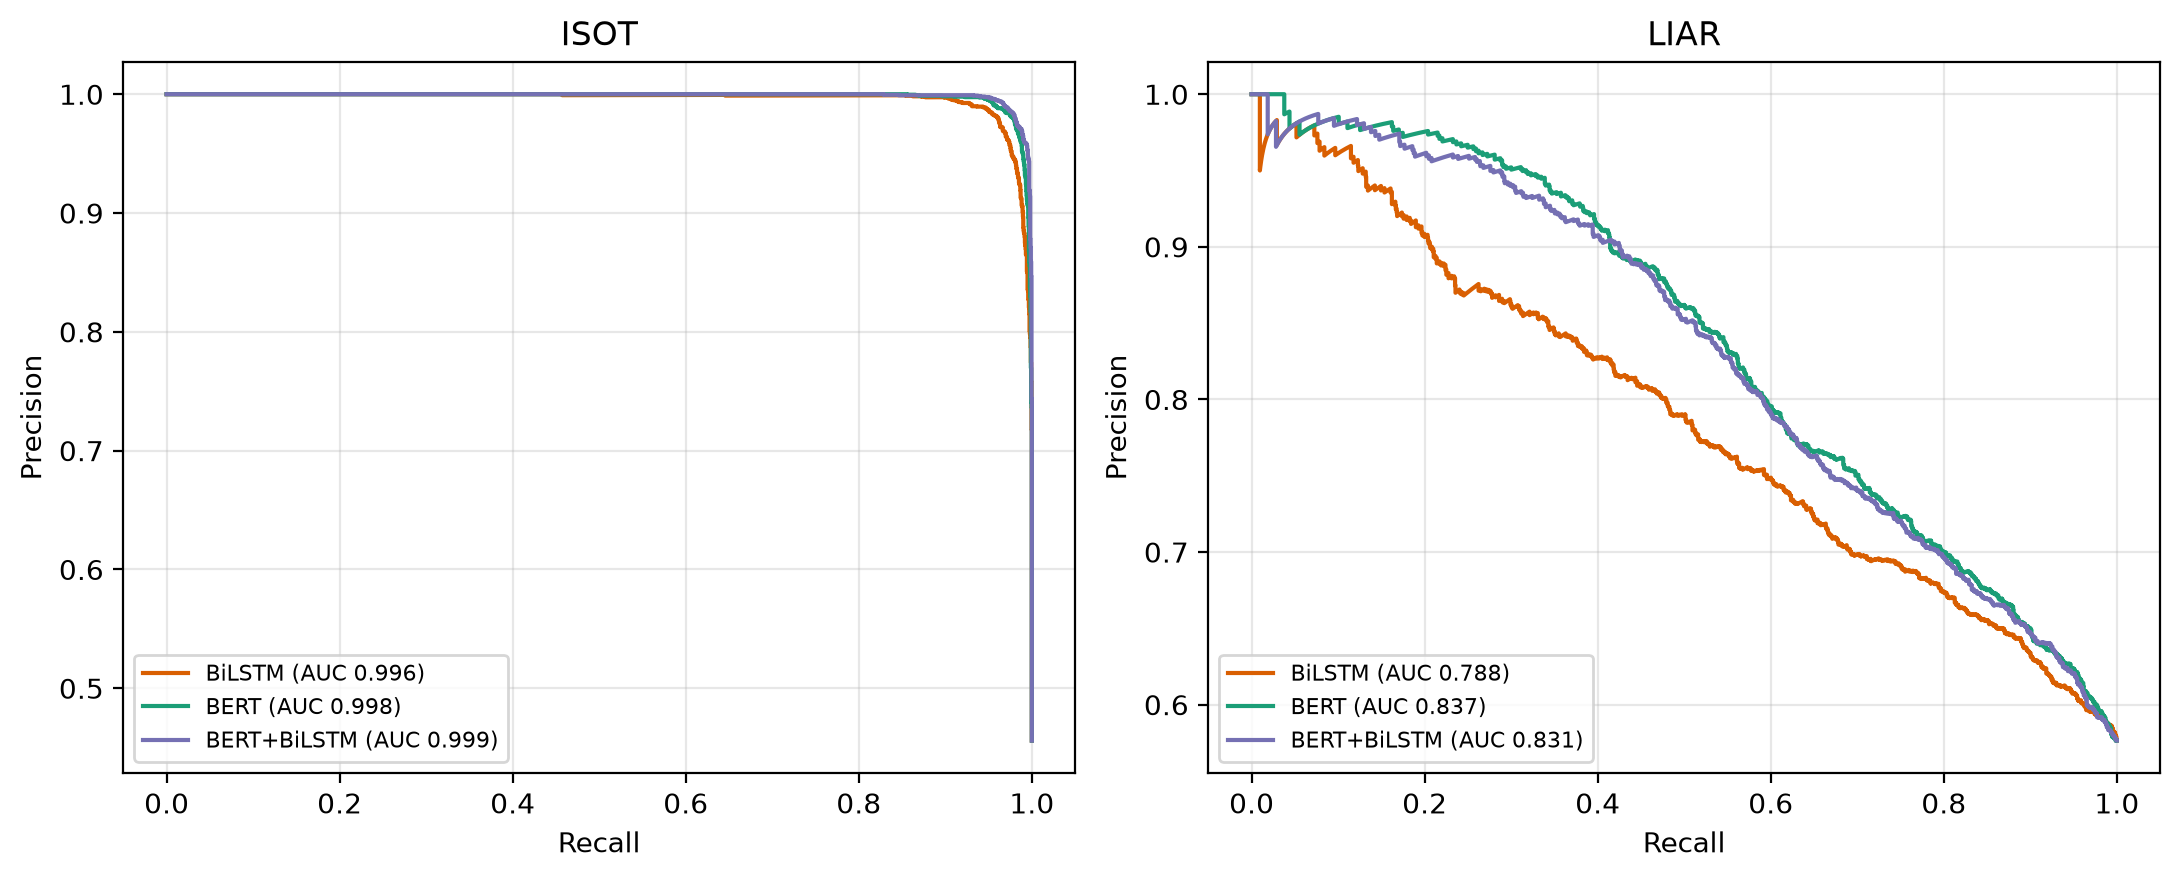
\includegraphics[width=\textwidth]{figures/PR Curve.png}
\caption{PR Curves for BERT, BiLSTM and BERT+BiLSTM Model for all the datasets}
\label{fig:pr_curve}
\end{figure}

The loss learning curve shows how well the model learned in each epoch. On ISOT the validation loss of BERT + BiLSTM is lowest at epoch 2 (0.060) and rises slightly at epoch 3 (0.067) while the training loss keeps falling. On LIAR2 the same model has its lowest validation loss after epoch 1 (0.566) and then rises to 0.594, so it starts to overfit after one epoch on the harder dataset. Fig. 5 shows the loss curves of BERT, BiLSTM, and BERT+BiLSTM for both datasets.

\begin{figure}[htbp]
\centering
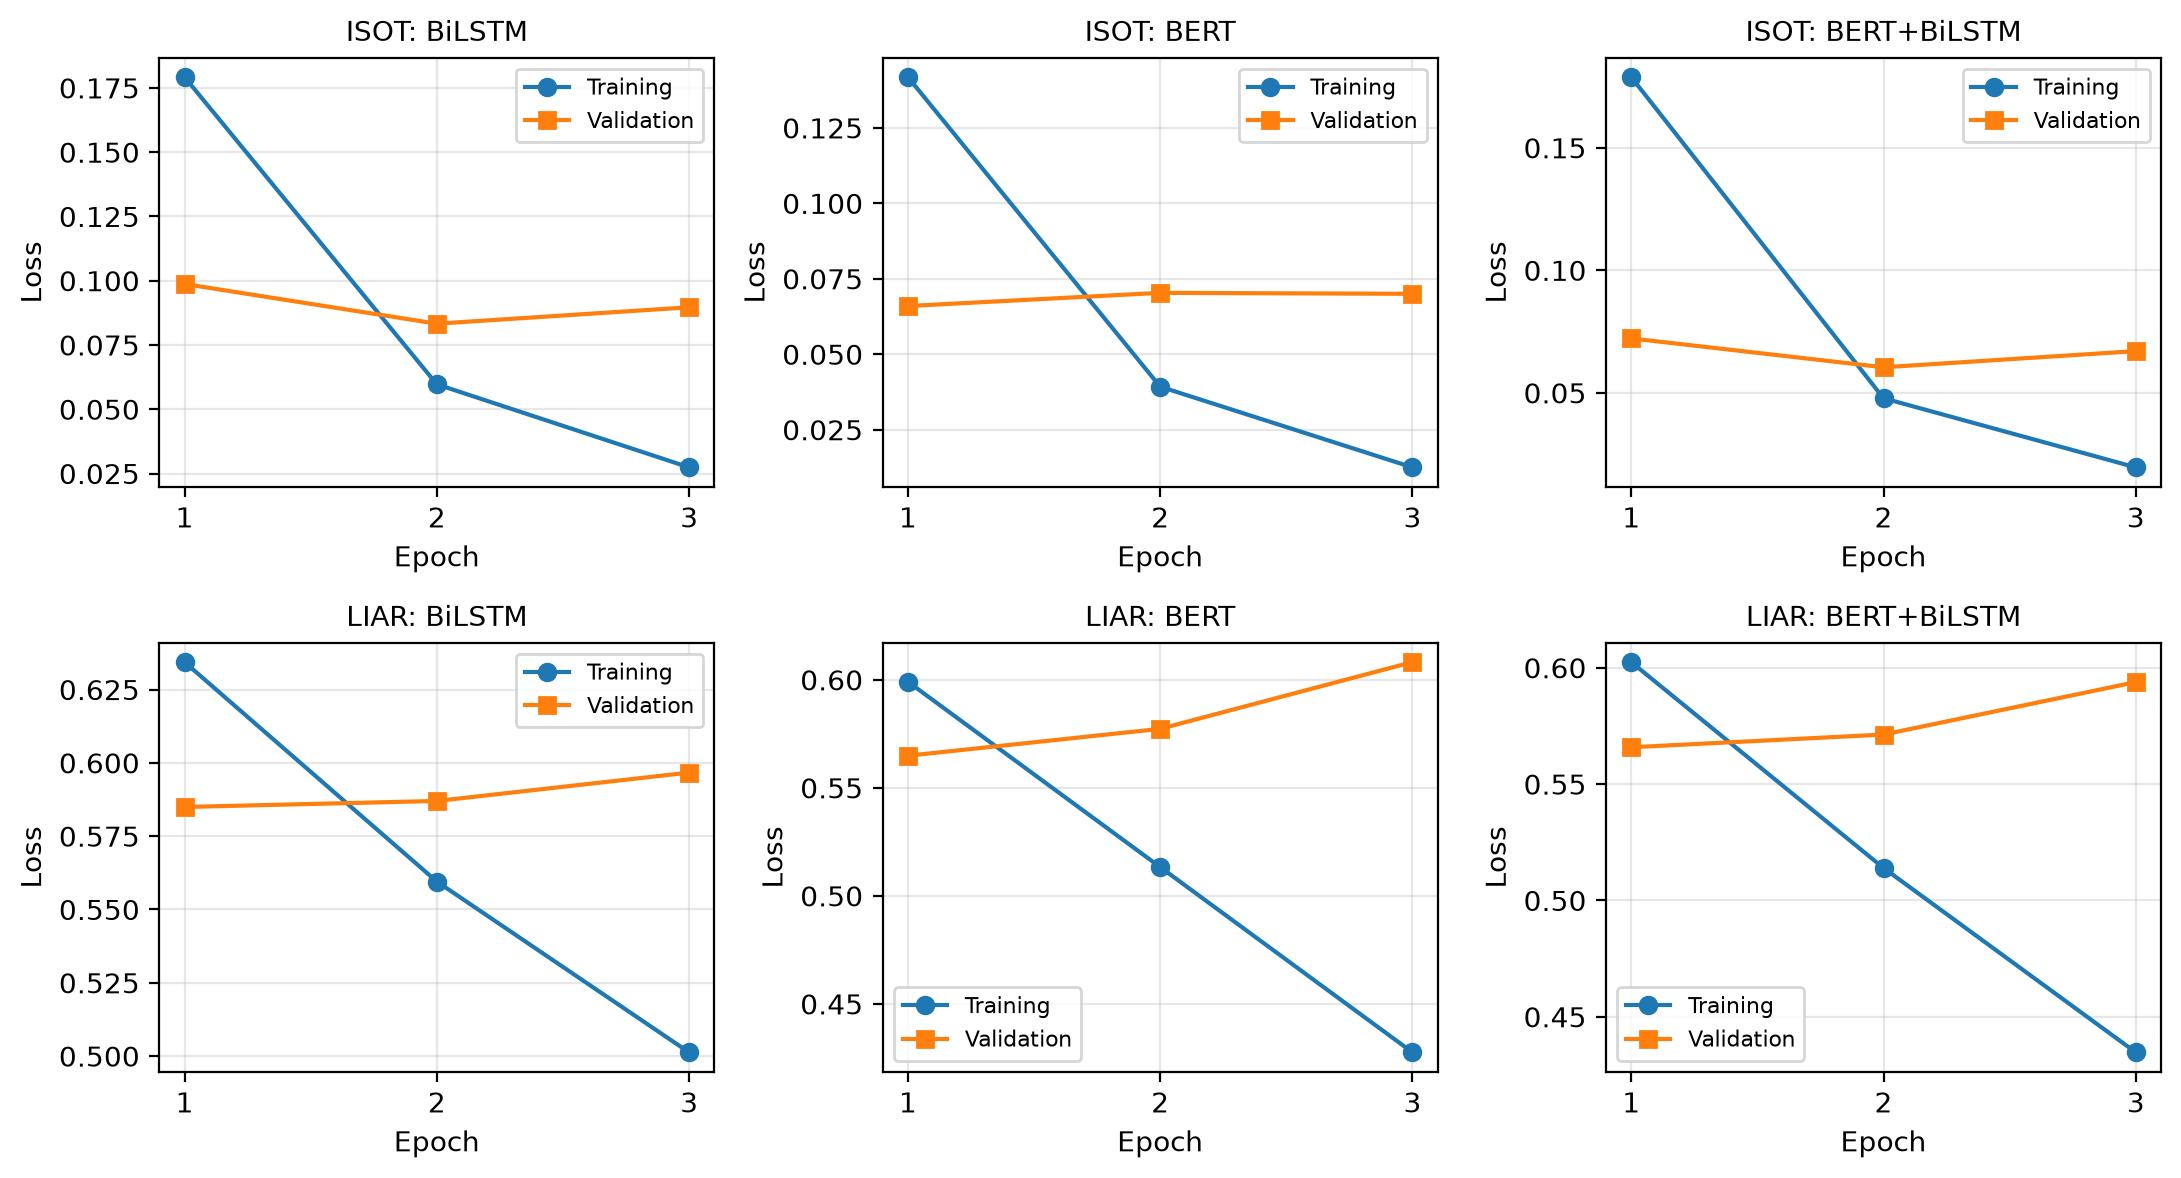
\includegraphics[width=0.88\textwidth]{figures/Loss.jpg}
\caption{Loss Curves for BERT, BiLSTM and BERT+BiLSTM Model for all the datasets}
\label{fig:loss}
\end{figure}

\subsection{Preliminary Zero-Shot Evaluation with a Local LLM}

As a first step toward the LLM direction named as future work in Section 5, a zero-shot experiment was run with a locally hosted large language model instead of the fine-tuned classifiers above. The open-weight instruction-tuned model Qwen2.5-1.5B-Instruct \cite{Yang2024Qwen25} ran entirely on a local CPU through the Hugging Face \texttt{transformers} library \cite{Wolf2020Transformers}, with no fine-tuning, no retrieval augmentation, and no task-specific training. For each article, the model received the headline and a truncated excerpt of the body in a system prompt that told it to answer with exactly one word, REAL or FAKE. The output was parsed and compared with the ground-truth label.

The test used a stratified random sample of 300 articles (150 real, 150 fake) from the same ISOT-derived corpus \cite{ISOTDataset} used elsewhere in this study. The results are comparable in kind, though not in scale, with Table \ref{tab:comparison}. Table \ref{tab:llm-comparison} gives the metrics.

\begin{table}[H]
\centering
\caption{Zero-Shot Performance of a Local LLM Compared to Fine-Tuned Models}
\label{tab:llm-comparison}
\small
\begin{tabular}{|l|c|c|c|c|}
\hline
\textbf{Model} & \textbf{Accuracy} & \textbf{Precision} & \textbf{Recall} & \textbf{F1 Score} \\ \hline
BiLSTM (fine-tuned, ISOT) & 0.9714 & 0.9846 & 0.9523 & 0.9682 \\
BERT (fine-tuned, ISOT) & 0.9768 & 0.9886 & 0.9603 & 0.9742 \\
BERT + BiLSTM (fine-tuned, ISOT) & 0.9815 & 0.9914 & 0.9679 & 0.9795 \\
Local LLM, Qwen2.5-1.5B-Instruct (zero-shot) & 0.7233 & 0.9136 & 0.4933 & 0.6407 \\ \hline
\end{tabular}
\end{table}

Without any task-specific training, the zero-shot LLM reaches 72.33\% accuracy. That is well above chance and clearly below the fine-tuned transformers. Its precision (0.9136) is high, so articles it flags as FAKE are usually fake. Its recall (0.4933) is low: it misses about half of the fake articles and answers REAL whenever the writing style shows no obvious red flag. This pattern fits a model that judges surface style and not verified evidence, since a well-written fabrication can look the same as genuine reporting without external fact-checking signals.

These preliminary results support the RAG-based direction outlined in the Future Scope discussion. Grounding the LLM's decision in evidence retrieved from sources such as Snopes, PolitiFact, or Wikipedia, and not in stylistic judgement alone, would be expected to improve recall on subtler fake articles.

\subsection{GRU-Based Hybrid Architectures}

To see whether lighter recurrent architectures can approach the transformer results, a standalone Gated Recurrent Unit (GRU) model and four GRU-based hybrids were trained on the ISOT-derived Kaggle corpus (23,481 fake and 21,417 real articles). The input was the headline only. Headlines were lower-cased, stripped of non-alphanumeric characters and stopwords, tokenized with a 10,000-word vocabulary (12,000 for GRU+BiLSTM), and padded or truncated to 40 tokens. A stratified 70:15:15 split gave 31,428 training, 6,735 validation, and 6,735 test samples. All models used the Adam optimizer (learning rate $10^{-3}$), binary cross-entropy loss, batch size 64, dropout 0.3, and at most 12 epochs, with early stopping on validation loss (patience 3, best weights restored).

The five architectures are: (i) a single GRU layer followed by global max-pooling over all time steps; (ii) a GRU followed by an LSTM layer; (iii) a 1D convolution and pooling stage feeding a GRU; (iv) a GRU followed by a Bidirectional LSTM; and (v) two 1D residual convolutional blocks feeding a GRU. Table \ref{tab:gru-comparison} gives the test-set results.

\begin{table}[H]
\centering
\caption{Test Performance of GRU and GRU-Hybrid Models (Headline-Only Input)}
\label{tab:gru-comparison}
\small
\begin{tabular}{|l|c|c|c|c|c|}
\hline
\textbf{Model} & \textbf{Loss} & \textbf{Accuracy} & \textbf{Precision} & \textbf{Recall} & \textbf{F1 Score} \\ \hline
GRU + BiLSTM & 0.1202 & 0.9546 & 0.9694 & 0.9429 & 0.9560 \\
GRU & 0.1249 & 0.9531 & 0.9596 & 0.9503 & 0.9549 \\
GRU + CNN & 0.1253 & 0.9534 & 0.9685 & 0.9415 & 0.9548 \\
GRU + LSTM & 0.1290 & 0.9520 & 0.9454 & 0.9640 & 0.9546 \\
GRU + ResNet & 0.1179 & 0.9513 & 0.9672 & 0.9387 & 0.9528 \\ \hline
\end{tabular}
\end{table}

\begin{figure}[htbp]
\centering
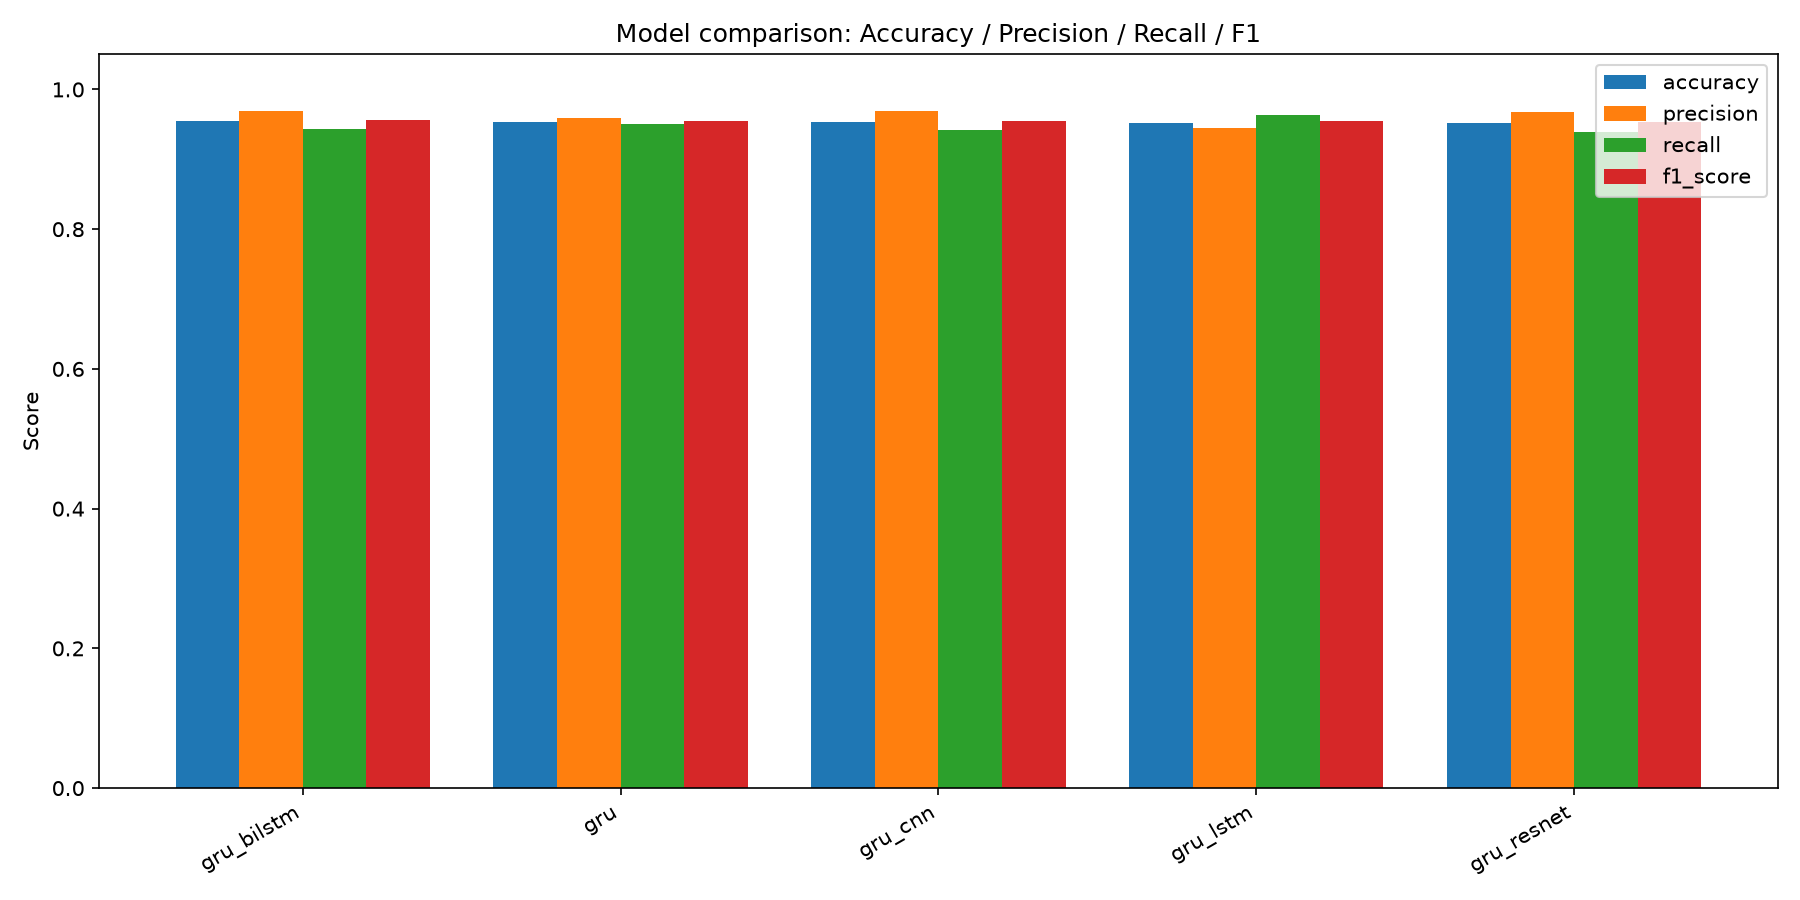
\includegraphics[width=0.88\textwidth]{figures/comparison_metrics.png}
\caption{Accuracy, Precision, Recall and F1 Score of the GRU and GRU-Hybrid Models}
\label{fig:gru_metrics}
\end{figure}

The five models lie within 0.4 percentage points of each other in accuracy and 0.33 points in F1, so the extra convolutional, residual, or second recurrent stage gives no meaningful gain over the standalone GRU. GRU+BiLSTM has the highest F1 (0.9560) and GRU+ResNet the lowest test loss (0.1179), but the differences are small. The hybrids trade precision against recall: GRU+BiLSTM has the highest precision (0.9694) and GRU+LSTM the highest recall (0.9640). The standalone GRU collapsed to the majority class when only its final hidden state was used, and pooling over every time step fixed this. GRU+ResNet trained less stably, and its validation accuracy dropped to 0.7526 at one epoch before it recovered. Trained on short headlines with a small vocabulary, these models reach accuracy close to that of the fine-tuned BERT models in Table \ref{tab:comparison} while being far smaller.

\subsection{Cross-Dataset Generalization}
The in-domain scores above come from ISOT, whose headlines carry source artifacts such as the ``(Reuters)'' tag. To test whether the models learn the news content and not these markers, we removed source tags and URLs, dropped duplicate titles, split each dataset 70/15/15 with stratification, and trained on one dataset while testing on the other. The second dataset is LIAR2, with labels 0--2 treated as fake and 3--5 as real. Every setting was repeated over three random seeds (five for the GRU). Table \ref{tab:cross-dataset} gives the mean and standard deviation.

\begin{table}[htbp]
\centering
\caption{Cross-dataset results (mean $\pm$ std over seeds). Cross-domain rows use the full other dataset as the test set.}
\label{tab:cross-dataset}
\begin{tabular}{llllll}
\hline
Model & Train & Test & Accuracy & F1 & AUC \\
\hline
GRU & ISOT & ISOT (in-domain) & 0.962 $\pm$ 0.001 & 0.958 $\pm$ 0.002 & 0.993 \\
GRU & ISOT & LIAR2 (cross) & 0.532 $\pm$ 0.009 & 0.662 $\pm$ 0.013 & 0.466 \\
GRU & LIAR2 & LIAR2 (in-domain) & 0.680 $\pm$ 0.006 & 0.725 $\pm$ 0.004 & 0.749 \\
GRU & LIAR2 & ISOT (cross) & 0.475 $\pm$ 0.008 & 0.627 $\pm$ 0.004 & 0.681 \\
BERT & ISOT & ISOT (in-domain) & 0.984 $\pm$ 0.002 & 0.982 $\pm$ 0.002 & 0.999 \\
BERT & ISOT & LIAR2 (cross) & 0.504 $\pm$ 0.001 & 0.611 $\pm$ 0.001 & 0.472 \\
BERT & LIAR2 & LIAR2 (in-domain) & 0.694 $\pm$ 0.004 & 0.733 $\pm$ 0.013 & 0.770 \\
BERT & LIAR2 & ISOT (cross) & 0.460 $\pm$ 0.002 & 0.626 $\pm$ 0.001 & 0.562 \\
BERT & ISOT + LIAR2 & ISOT (in-domain) & 0.984 $\pm$ 0.001 & 0.982 $\pm$ 0.001 & 0.998 \\
BERT & ISOT + LIAR2 & LIAR2 (in-domain) & 0.693 $\pm$ 0.004 & 0.717 $\pm$ 0.009 & 0.772 \\
\hline
\end{tabular}
\end{table}

Three findings follow. First, both models separate ISOT almost perfectly in-domain (BERT AUC 0.999) but fall to chance on LIAR2 (accuracy 0.50, AUC 0.47), and a model trained on LIAR2 falls below chance on ISOT. The high in-domain accuracy therefore reflects dataset-specific patterns more than transferable cues of fake news. Second, BERT gains only a little over the GRU on LIAR2 (F1 0.733 against 0.725), so a larger encoder does not fix the problem on its own. Third, training on both datasets keeps ISOT accuracy at 0.984 and LIAR2 AUC at 0.772, so mixing sources costs nothing in-domain, but this has not yet been tested on a third, unseen dataset. The LIAR2 rows in Table \ref{tab:comparison_extended} come from a single seed and a 70:15:15 split, so they differ slightly from the three-seed means used in the cross-dataset table (BERT 0.694 accuracy). Closing the cross-domain gap is the main remaining work: stronger encoders, article-body input, retrieval-augmented classification, and explainability checks.

\section{Conclusion and Future Research Directions}

This study examined a transformer-based approach to fake news identification and compared several classical and neural network models. It evaluated the BiLSTM, BERT, and a hybrid of BERT and BiLSTM for detecting fake news.

Across the experiments on ISOT, the BiLSTM, BERT, and BERT + BiLSTM reached 97.1\%, 97.7\%, and 98.2\% accuracy, with F1 scores of 0.968, 0.974, and 0.980. The hybrid was meant to combine contextual and sequential learning, and it gave a small gain on ISOT only. On LIAR2 the three models reached 66.4\%, 68.9\%, and 68.2\% accuracy, and BERT alone was the best. The gaps between models are small and come from one seed, so the main conclusion is that the choice of model matters less than the choice of dataset.

Within each dataset, transformer-based models gave stable results. BERT alone is the best choice for implementation, since it performs at a high level without added complexity.

A further comparison of a standalone GRU with four GRU-based hybrids (GRU+LSTM, GRU+CNN, GRU+BiLSTM, GRU+ResNet) on headline-only input gave accuracies of 95.1--95.5\% and F1 scores of 0.9528--0.9560 (Table \ref{tab:gru-comparison}). The hybrids offer no meaningful advantage over the standalone GRU, and all of them come close to the fine-tuned BERT models while being far smaller.

LLMs and XAI techniques are not part of the main system design. A preliminary zero-shot experiment with a local LLM (Section 4, Table \ref{tab:llm-comparison}) reached 72.33\% accuracy without any task-specific training, but its recall was far lower than that of the fine-tuned transformers. This motivates the RAG and evidence-grounding directions discussed below and does not replace the fine-tuned pipeline.

A cross-dataset test with cleaned and deduplicated headlines shows the limit of the in-domain scores. Trained on ISOT, BERT reaches 0.984 accuracy on ISOT but only 0.504 on LIAR2, and the GRU behaves the same way (0.532). The models therefore learn dataset-specific patterns more than transferable cues of fake news. Training on ISOT and LIAR2 together keeps ISOT accuracy at 0.984 and gives a LIAR2 AUC of 0.772, but this has not yet been tested on a third dataset. The main work that remains is to close this gap with stronger encoders, article-body input, retrieval-augmented classification, and explainability analysis.

\subsection{Future Scope}

Future work should investigate more advanced large language models such as GPT-4, LLaMA 2, Mistral, and Gemini in the detection pipeline. Retrieval-Augmented Generation (RAG) would let the model use verified databases such as Snopes, PolitiFact, and Wikipedia to find evidence in real time before classifying information. This would improve performance and reliability when misinformation takes complicated forms such as satire, propaganda, and contextual misinformation.

The main limitation of deep learning models is that they work as black boxes, which makes it hard for users to understand why a decision was made. Future work should add eXplainable AI (XAI) approaches for transparency. In such a framework, an LLM, possibly helped by evidence retrieval, first classifies the input document, and a further layer then generates a human-readable explanation of the prediction. This is expected to give both good accuracy and interpretability for users such as journalists and fact-checkers. We will also address deployment issues: multilingual detection, multi-modal fake news analysis, federated learning, and an API.
\bibliographystyle{splncs04}
\bibliography{references}

\end{document}